
%%% Local Variables:
%%% mode: latex
%%% TeX-master: "../thesis"
%%% End:

\chapter{Strongly correlated materials}
\label{chap:cthyb}
\section{Introduction}

Many interesting phenomena in materials can be simply described in term
of a picture in which particles are independent from each others. For a periodic
system, Bloch's theorem, provides the basis for the description of materials
in term of band structure. The energy eigenstates can be expanded in term
of the periodic function with definite momentum number. Even such a seemingly
simple independent particle picture harbors a vast amount of interesting phenomena.
Nine decades have passed after the Bloch's theorem, the physics of non-interacting electrons are
still being investigated intensively today. The exotic physics, such as 
the topological structure of the band theory still have not been exhausted,
typical examples include quantum hall effect and topological insulators.

Effects from interaction among particles cannot be completely ignored in many
interesting systems. The physics can quickly becomes very complicated when
the interaction becomes a dominating factors in the system. Unlike the simple
single particle picture, there is no generic efficient method for the study 
of quantum interacting systems. From a computational point of view, the size
of the quantum system, Hilbert space, grows exponentially as the number of 
particles. It is in general very difficult to analyze such systems by simple numerical mean.

However if one can reduce the systems into a somewhat single particle like systems,
the analysis can be greatly simplified. The Landau Fermi liquid theorem, a landmark
achievement in the study of correlated systems, tells us that in many
circumstances the interacting system can be reduced into a single particle system with
some modifications. The non-interacting particle can be adiabatically deformed
into quasi-particle with a finite lifetime. This important prediction by Landau
can only be explained few decades later when the concepts of renormalization group
of fermion systems are applied in the condensed matter physics.

Although the Fermi liquid theorem can satisfactory explained a lot of metallic
system, its limitation is obvious. It fails in the low-dimensional
cases, by now, we know that this is invalid in one dimension. However, the question 
of its validity in two dimension is more subtle. As many of the interesting systems, their
physics are believed to be largely dictated by the correlation in two dimension.
This is also the main battlefield of strongly correlated system. In one dimension, 
various rather accurate numerical methods are available; in higher dimension, 
mean field theory is presumably a good starting point. At two dimension, there is 
usually no good control on analytical calculations, and numerical methods on lattice
models are hindered by the minus sign problem in Quantum Monte Carlo or the lack
of good renormalization of the Hilbert space. Another clear deficit of the Fermi liquid 
theory is its inability to describe the quantum criticality, It is obvious that the 
criticality involve collective behaviors. An independent particle picture is 
doomed to fail in describing critical points. Further increase the interaction, 
the independent particle picture in the momentum space has to be replaced by the Mott 
picture in the real space, and there is no adiabatic continuation which can tune
the single particle metallic system into a real space picture of Mott insulator.

Thus a systematic, even though approximated, method is sought for the study of strong correlation. 
The method which can describe the physics from metallic, to critical, to insulating phase as 
the interaction is cranked up is crucial for the study of strongly correlated systems. 
We will discuss in the following that the dynamical mean field method and its cluster extension, 
dynamical cluster approximation, fulfilled such a request. Combining with the density functional theory,
a semi-quantitative numerical results can sometimes be obtained for strongly correlated materials. 


In a sense, from the above discussion, the term strong correlation refers to the behavior of electrons
that cannot be well-described by simple one-electron theories. Materials
which naturally have a tendency of strongly correlation are those involved
unfilled d or f orbitals. This is due to the small orbital radius of
$d$ and $f$ orbitals and so does the overlap among orbitals.
This reduces the kinetic energy of the system, the electrons are said to be living 
in the narrow band, and thus the interaction becomes more important. Many interesting materials discovery which host
a range of interesting experimental observations, the most prominent example is the
high temperature conductivity, pseudogap behaviors, quantum
criticality, in the past few decades involve transition
metal or inner transition metal. This is precisely because of the effective
strong correlation due to the $d$ or $f$ orbitals.

Understanding those exotic behaviors is extremely challenging. There is a major
obstacles. Once the single particle picture fails, there
is no good starting point for many perturbative calculations. It renders
into a regime almost all analytical methods will fail. In the following we 
will discuss two majors progress in attacking correlated systems. The first one 
is DFT, a many-site single particle treatment; and the other one is DMFT, a single site 
many-body treatment. 

\section{Numerical approaches in strongly correlated materials}
Numerical calculation in strongly correlated fermion systems is a major 
challenge in condensed matter physics. In real world, materials consists of 
$10^{23}$ interacting particles, which is impossible to solve at first glance. 
Fortunately, not all the particles contribute to the property of materials. For 
example, in a metal only the electrons close to the Fermi level can be excited 
and contribute ,e.g., to the transport and magnetic properties. In a lattice, 
lattice excitations are few at low T, but they are responsible for inelastic 
neutron scattering. Even though, the remaining problem is still hard. 

Density functional theory (DFT)\cite{PhysRev.136.B864,PhysRev.140.A1133} 
provides a framework to solve the 
electron structure problem. Using this theory, the properties of a many-electron
system can be described by a functional of election density. Combined with 
approximations that address the exchange-correlations such as the local density 
approximation (LDA) \cite{lundqvist1983}, DFT produces satisfactory data that agrees well the 
experiments for many cases. However, despite the success in weakly correlated 
materials, there are still difficulties in applying this method to other 
cases, such as systems with strongly correlation \cite{0953-8984-9-35-010}. 
The accuracy of DFT has seen gradually improve over the year, the continual
development in functional to include correction from beyond local density 
plays an important part. However, it seems to be quite
difficult to handle such strong correlation by simple improvements of the 
DFT. A promising direction is to combine other methods which can treat
strong correlation with the DFT method. A popular choice is to employ 
the dynamical mean field theory\citep{RevModPhys.68.13,PhysRevB.45.6479} (DMFT)
to include the effect from the electron-electron
correlation on top of the single particle dispersion obtained from the DFT. 

%DFT, ab inito

%maybe mention other numerical methods here?

DMFT has been widely used on a range of strongly correlated systems. 
It is a method well suited for strongly correlated systems, in particular it 
captures the Mott transition, a hallmark of strong correlation, of the Hubbard 
model. In this approach, the solution of the lattice model is mapped to a 
quantum impurity model with self-consistency conditions. 
%intro to impurity
%mention other impurity solvers
A quantum impurity problem describes an atom embedded in a host medium. 
The impurity consists of a set of orbitals with different parameters, populated
with electrons that interacts with each other. The orbitals are hybridized to 
bath orbitals representing the degrees of freedom of the host materials. 
The solution of impurity problem can be obtained in a few different ways. 
We will focus on the different variants of Monte Carlo methods.

A commonly used technique is the Hirsch-Fye method \cite{1986PhRvL..56.2521H}, in which a 
Hubbard-Stratonovich transformation is used to decouple the interaction part,
leading to determinants which give the weights associated with the 
configurations of the auxiliary fields, which are then sampled by a Monte Carlo 
procedure. One issue is that Hirsch-Fye cannot be easily applied to complicated
interaction that include more than just density-density interaction, due to the
lack of simple ansatz to decouple the interacting terms. 
The matrix size scales to the interaction as well as the inverse of 
temperature, which makes the calculation inefficient at low temperatures.
This methods also requires discretization of the imaginary time interval,
which introduce systematic errors, and may not be optimal for multi-orbital case 
with complicated off-diagonal couplings.

The Trotter error in Hirsch-Fye algorithm can be eliminated by using the 
Continuous Time Monte Carlo algorithms. For example, one can solve the problem 
exactly in non-interacting limit, and treat the interaction with a Taylor-series
 expansion. By doing stochastic sampling of diagrams in the weak-coupling 
expansion of partition function, the interaction expansion (CT-INT) algorithm
\cite{2005PhRvB..72c5122R}
provides a discretization error free alternative Hirsch-Fye algorithm.
Still, in the CT-INT algorithm, it is difficult to treat non-Hubbard-type 
interactions. Also the size of the matrix used in the CT-INT method grows
quickly with the interaction, making the calculation very time-consuming at 
very strong interactions.

Another way to treat the impurity problem is the hybridization expansion (CT-HYB)
approach \cite{RevModPhys.83.349, PhysRevB.75.155113, PhysRevB.80.235117,
PhysRevB.74.155107}. 
The fact that the order of expansion decreases with increasing 
interaction makes this method favorable for strong interaction systems. 
The algorithm is also found to work at very low temperatures, and is applicable
to a wider class of impurity models including those with complicated 
off-diagonal couplings, since the local problem is treated exactly. 

\section{Algorithm}
\label{sec:hyb-alg}
\subsection{Hybridization Expansion CTQMC algorithm}
A quantum impurity model may be represented as a Hamiltonian $H_\text{QI}$

\begin{equation}
H_\text{QI}=H_\text{loc}+H_\text{bath}+H_\text{hyb}
\end{equation}
\begin{eqnarray}
H_\text{loc}&=& H_\text{loc}^0+H_\text{loc}^I=
                \sum_{ab} E^{ab}d^\dagger_a d_b + 
                \sum_{pqrs}I^{pqrs}d^\dagger_p d^\dagger_q d_r d_s \\
H_\text{bath}&=&\sum_{k\alpha} 
                 \varepsilon_{k\alpha}c^\dagger_{k\alpha}c_{k\alpha} \\
H_\text{hyb}&=&\sum_{k\alpha b} ({V}_k^{\alpha b}c^\dagger_{k\alpha}d_b 
                +\text{h.c.})
\end{eqnarray}

$H_\text{loc}$ describes the ``impurity'' (a system
with a finite (typically small) number of degrees of freedom), 
$H_\text{bath}$ describes the non-interacting system, 
and $H_\text{hyb}$ gives the coupling between the impurity and bath.

The Anderson impurity model describes a localized electronic level, subject to 
a local Coulomb interaction, which is coupled to a band of non-interacting 
conduction electrons. In the  single-impurity single-orbital case, its 
Hamiltonian is given by
\begin{equation}
H_\text{AIM}= \underbrace{\sum_{k\sigma}
  \varepsilon_k c^\dagger_{k\sigma}c_{k\sigma}}_{H_\text{bath}} 
+  \underbrace{\sum_\sigma \varepsilon_0d^\dagger_\sigma d_\sigma 
  + Un_\uparrow n_\downarrow}_{H_\text{loc}}
+ \underbrace{\sum_{k\sigma}\Big(V_kc^\dagger_{k\sigma}d_\sigma+h.c.\Big)}
_{H_\text{hyb}}
\end{equation}


In Hybridization Expansion Continuous Time Quantum Monte Carlo (CT-HYB)
\cite{RevModPhys.83.349,PhysRevB.75.155113,PhysRevB.80.235117,
PhysRevB.74.155107}, 
we take the hybridization term as a perturbation, i.e.
\begin{equation}
H_b=H_\text{hyb} = \sum_{pj} (V_p^j c_{p}^\dagger d_j
+ \sum_{pj} V_p^{j*}d_j^\dagger c_{p})
\end{equation}
and thus the partition function becomes
\begin{align}
Z &=\sum_{k=0}^\infty\int_0^\beta d\tau_1 \ldots \int_{\tau_{k-1}}^\beta d\tau_k 
    \int_0^\beta d\tau_1' \ldots  \int_{\tau_{k-1}'}^\beta d\tau_k' 
\sum_{\substack{j_1, \cdots j_k\\j_1', \cdots j_k'}}\sum_{\substack{p_1, \cdots p_k\\p_1',\cdots p_k'}} V^{j_1}_{p_1}V^{j_1'*}_{p_1'} \cdots V^{j_k}_{p_k}V^{j_k'*}_{p_k'}  \nonumber\\
&\times\Tr_d\left[T_\tau e^{-\beta H_\text{loc}} d_{j_k}(\tau_k) d_{j_k'}^\dagger(\tau_k')\cdots d_{j_1}(\tau_1)d_{j_1'}^\dagger(\tau_1')\right] \nonumber\\
&\times\Tr_c\left[T_\tau e^{-\beta H_\text{bath}} c^\dagger_{p_k}(\tau_k)c_{p_{k'}}(\tau_k')\cdots c_{p_1}^\dagger(\tau_1) c_{p_1'}(\tau_1')\right]
\end{align}
The bath partition function could be integrated out
\begin{align}
Z_\text{bath} = \Tr e^{-\beta H_\text{bath}} = \prod_\sigma \prod_{p} (1+e^{-\beta \varepsilon_{p}}),
\end{align}
With the anti-periodic hybridization function $\mathbf{\Delta}$,
\begin{align}
\Delta_{lm}(\tau) = \sum_p \frac{V^{l*}_p V^m_p}{e^{\varepsilon_p\beta}+1} \times 
\left\{ 
\begin{array}{ll}-e^{-\varepsilon_p(\tau-\beta)},& 0<\tau<\beta \\ 
e^{-\varepsilon_p\tau},&  -\beta<\tau<0\end{array}
\right.,
\end{align}
and by separating the contributions from each spin, we obtain
\begin{equation}
\label{partition_function}
Z =  Z_\text{bath}\prod_j \sum_{k_j=0}^\infty \int_0^\beta d\tau^j_1 \ldots \int_{{\tau'}^j_{k_j-1}}^\beta d{\tau'}^j_{k_j} 
\times \Tr_d\Big[T_\tau e^{-\beta H_\text{loc}} d_j(\tau^j_{k_j}) d_j^\dagger(\tau'^j_{k_j})\ldots d_j(\tau^j_{1})d_j^\dagger(\tau'^j_1)\Big] \det \mathbf{\Delta}_j
\end{equation}

Where 
\begin{equation}
  \label{eq:hyb-matrix}
  \Delta=\left[
    \begin{array}{cccc}
      \Delta(\tau_0'-\tau_0) & \Delta(\tau_0'-\tau_1) & \cdots & \Delta(\tau_0'-\tau_n)\\
      \Delta(\tau_1'-\tau_0) & \Delta(\tau_1'-\tau_1) & \cdots & \Delta(\tau_1'-\tau_n)\\
      \cdots & \cdots & \cdots & \cdots \\
      \Delta(\tau_n'-\tau_0) & \Delta(\tau_n'-\tau_1) & \cdots & \Delta(\tau_n'-\tau)\\
    \end{array}
  \right]
\end{equation}


We can sample the partition function above using Monte Carlo method. To 
determine the weight of each configuration, we need to calculate the contribution
from the local part (the trace) and the hybridization part (the determinant).
We would discuss both in the following sections \ref{sec:trace_segment},
\ref{sec:trace},\ref{sec:hyb_matrix}, and introduce scalable 
algorithms in \ref{sec:cthyb_krylov} and \ref{sec:cthyb_fmu}

\subsection{Evaluation of the trace using the segment picture}
\label{sec:trace_segment}
The trace factor represents the impurity with particles hopping in and out at 
imaginary times $\tau'$ and $\tau$, and the determinant sums up all compatible 
hybridization events with the bath. 
In the impurity basis ($\ket{0}$,$\ket{\uparrow}$,$\ket{\downarrow}$,
$\ket{\uparrow\downarrow}$) the Hubbard Hamiltonian is diagonal, 
and the creation and annihilation operators for given spin have to alternate 
for the trace to be finite. This allows the configuration of the operators to be
represented in a segment picture, where each pair of neighboring creation/annihilation 
operators is represented by a segments on the imaginary time axis, as shown in 
figure~\ref{fig:seg}.

%put segment picture here.
\begin{figure}[ht]
  \centering
  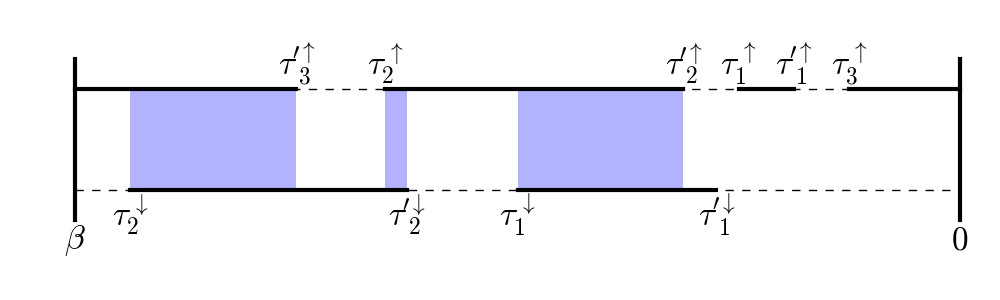
\includegraphics[width=0.8\textwidth] {img/segment.png}
  \caption{A segment picture showing a possible configuration of the two spin 
    channels. 
    The blue section indicates the overlap between two spin channels, 
    $l_\textrm{overlap}$ in eq.\ref{eq:weight_local}.}
\label{fig:seg}
\end{figure}


In the said basis, the contribution of the local Hamilton can be evaluated as:
\begin{equation}
\label{eq:weight_local}
W_{\textrm{loc}} = s_\uparrow s_\downarrow e ^{\mu(l_\uparrow+l_\downarrow)-Ul_{\textrm{overlap}}}
\end{equation}
Where $l_\sigma$ is the total length of segments on spin channel $\sigma$,
$l_{\textrm{overlap}}$ is the total overlap between two spin channels. The sign 
$s_\sigma$ is $-1$ when one of the segments winds around from $\beta$ to $0$, 
and $+1$ otherwise.

\subsection{Evaluation of the trace for non-diagonal Hamiltonian}
\label{sec:trace}
In models such as Dynamical Hubbard Model, the local part of Hamiltonian is not
diagonal in the occupation number basis, and therefore we cannot use the segment
picture to evaluate the trace easily. In this case We need to evaluate the 
trace of this term:
\begin{equation}
  \label{eq:1}
  e^{-H*(\beta-t_n)}F_{t_n}e^{-H*(t_n-t_{n-1})}F_{t_{n-1}}\ldots F_{t_0}e^{-Ht_0}  
\end{equation}
Where $H$ is the Hamiltonian, and $F_{t_{i}}$ is a Fermion operator at time $t_i$.

To evaluate the exponential terms, we diagonalize the Hamiltonian with
\[
H=UVU^T
\]
where $V$ is diagonal matrix with eigenvalues of $H$, each column of $U$ is a
eigenvector of $H$.
Using
\[
UU^T=I
\]
we have 
\[
e^{-Ht}=e^{-UVU^Tt}=Ue^{-Vt}U^T
\]
 the term becomes
\[
Ue^{-V*(\beta-t_n)}U^TF_{t_n}Ue^{-V*(t_n-t_{n-1})}\ldots F_{t_0}Ue^{-Vt_0}U^T
\]
define 
\[
D_t=U^TF_tU
\]
The term is then
\begin{equation}
  \label{eq:2}
  Ue^{-V*(\beta-t_n)}D_{t_n}e^{-V*(t_n-t_{n-1})}\ldots D_{t_0}e^{-Vt_0}U^T  
\end{equation}

We can then evaluate the full trace of the matrix above, using a series of 
matrix multiplications.


\subsection{Monte Carlo sampling}
\label{sec:cthyb_mcs}
To sample the configuration space with Monte Carlo procedures, one can propose 
a new configuration by:
\begin{itemize}
\item Adding a new segment to the existing configuration;
\item Removing a segment to the existing configuration;
\item Shifting an end of a segment in the existing configuration;
%\item Adding a new anti-segment to the existing configuration;
%\item Removing a anti-segment to the existing configuration;
\end{itemize}


To satisfy the detailed balance condition, we must make sure that 
\begin{equation}
W_{AB}/W_{BA}=W[B]W[A]
\end{equation}
where $A$ and $B$ are two configurations, and $W_{AB}$ is the transition
probability from configuration $A$ to configuration $B$, and vice versa.

In the case of adding a segment, one can first randomly choose a starting point 
for a segment, say $\tau'$ in $(\beta,0]$. If $\tau'$ falls on one of the 
existing segments, the proposal is rejected. Otherwise if $\tau'$ is located
between two segments $\tau_j$ and $\tau_{j+1}'$, we pick the end point from 
$[0,l_\textrm{max}]$, where 
$l_\textrm{max}=\mathrm{mod}(\tau_{j+1}'-\tau+\beta,\beta)$.
\begin{figure}[ht]
  \centering
  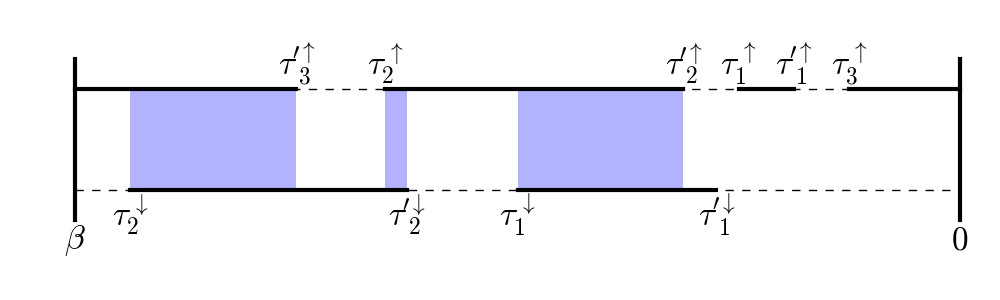
\includegraphics[width=0.8\textwidth] {img/segment.png}
  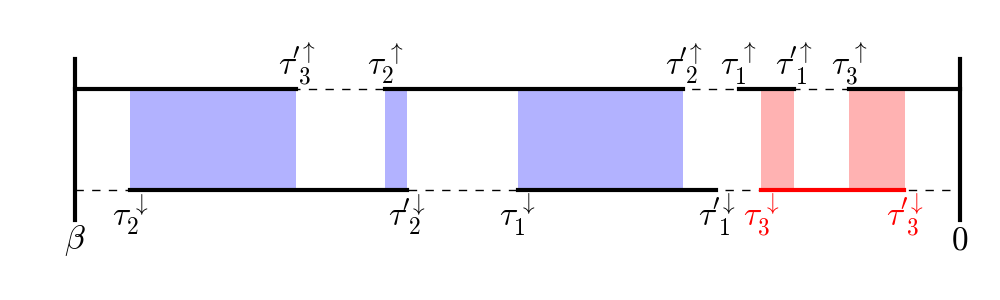
\includegraphics[width=0.8\textwidth] {img/segment_add.png}
  \caption{A segment picture showing the addition of a segment ($\tau_3',\tau_3$)
(red line) to the $\left|\downarrow\right\rangle$ channel. The red shade shows the
change of overlap from this addition.
}
\label{fig:seg_add}
\end{figure}
Assuming there is an infinitesimal grid with grid size $d\tau$ on the imaginary
time axis, the proposal probability can be found as:
\begin{equation}
P_\mathrm{prop:k\rightarrow k+1}=\frac{d\tau^2}{\beta\l_\mathrm{max}}
\end{equation}

\begin{figure}[ht]
  \centering
  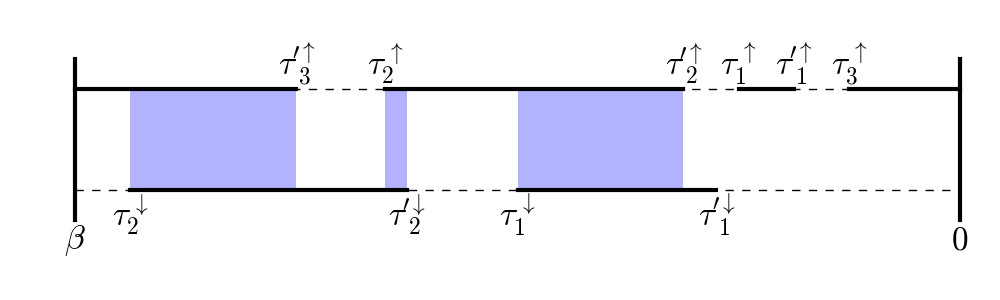
\includegraphics[width=0.8\textwidth] {img/segment.png}
  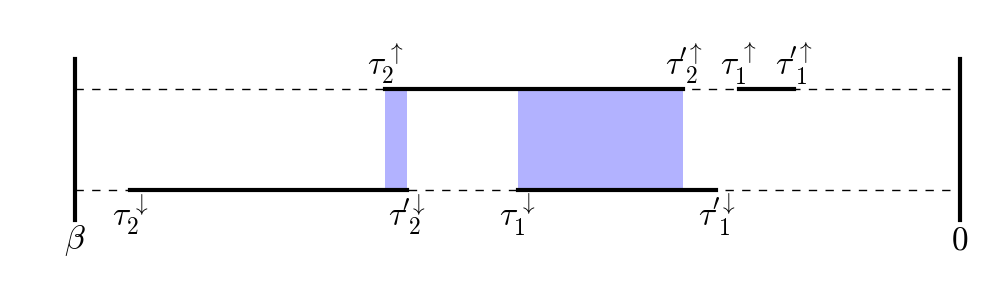
\includegraphics[width=0.8\textwidth] {img/segment_remove.png}
  \caption{A segment picture showing the removal of a segment ($\tau_3',\tau_3$)
(red line) from the $\left|\uparrow\right\rangle$ channel.
}

\label{fig:seg_remove}
\end{figure}
In the case of removing a segment, one can randomly pick a segment from $k_\sigma$ 
existing segments, and thus the proposal probability is 
\begin{equation}
P_\mathrm{prop:k\rightarrow k-1}=\frac{1}{k_\sigma}
\end{equation}

Combined with the detailed balance condition and previous weight calculations, 
we have the probability of accepting an addition as:
\begin{equation}
P_\mathrm{accpt:k\rightarrow k+1}=\min\left(1,\mathrm{sign}(\tau-\tau')
  \frac{\beta l_\mathrm{max}}{k_\sigma +1} \frac{\det\Delta^{k+1}}{\det\Delta^k}
  e^{\mu l}e^{-U \Delta l_\mathrm{overlap}}
\right)
\end{equation}
where $l$ is the length of segment to be added, and $\Delta l_\mathrm{overlap}$
is the change in overlap between two spin channels. 

Similarly, the acceptance ratio for removing a segment is:
\begin{equation}
P_\mathrm{accpt:k\rightarrow k-1}=\min\left(1,\mathrm{sign}(\tau-\tau')
  \frac{k_\sigma}{\beta l_\mathrm{max}} \frac{\det\Delta^{k-1}}{\det\Delta^k}
  e^{-\mu l}e^{U \Delta l_\mathrm{overlap}}
\right)
\end{equation}

\begin{figure}[ht]
  \centering
  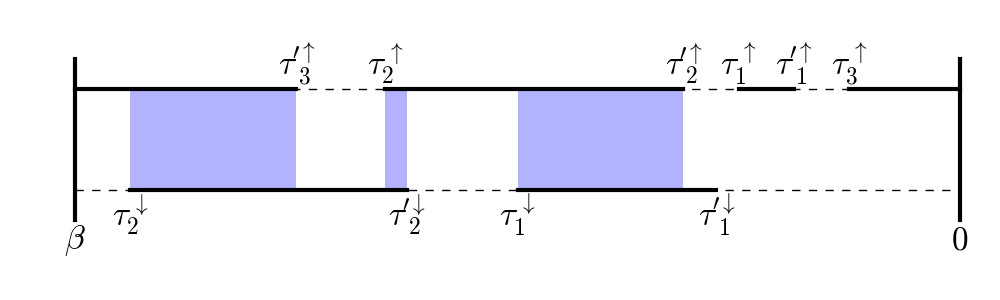
\includegraphics[width=0.8\textwidth] {img/segment.png}
  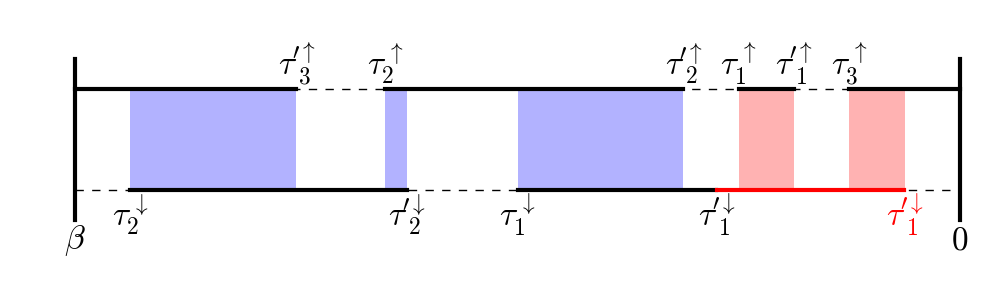
\includegraphics[width=0.8\textwidth] {img/segment_shift.png}
  \caption{A segment picture showing shifting the end of a segment ($\tau_1',\tau_1$)
(red line) on the $\left|\downarrow\right\rangle$ channel. The red shade shows the
change of overlap from this shift.
}

\label{fig:seg_shift}
\end{figure}

The probability for accepting a shifting move is:
\begin{equation}
P_\mathrm{accpt:k\rightarrow k}=\min\left(1,
  \mathrm{sign}(\tau_k-\tau_k')\mathrm{sign}(\tau_{k'}-\tau_{k'}')
  \frac{\det\Delta^{k}_{\mathrm{new}}}{\det\Delta^{k}}
  e^{\mu\Delta l}e^{-U \Delta l_\mathrm{overlap}}
\right)
\end{equation}

In the case where one or more channels has no segments, we need to evaluate the trace
from the Hamiltonian. Here $k$ refers to the number of segments on the channel
where the move is proposed, and $k'$ refers to the number of segments on the
channel with opposite spin direction.

\begin{enumerate}
  \item Adding a segments to channel $\sigma$.

    \begin{equation}
      P_\mathrm{accpt:k\rightarrow k+1}=\min\left(1,\mathrm{sign}(\tau-\tau')
        \frac{\beta l_\mathrm{max}}{k_\sigma +1} \frac{\det\Delta^{k+1}}{\det\Delta^k}
        *Q
      \right)
\end{equation}
where $Q$ is the ratio of the new trace verses the old trace. 

    \begin{enumerate}
    \item{$k=0,k'\neq 0$}

      \begin{equation}
        \label{eq:8}
        Q=
        \frac{e^{-l'_\sigma\epsilon_f}e^{-l_{ov}U}}
        {1+e^{-\beta\epsilon_f}e^{-l_{\bar\sigma} U}}
      \end{equation}
      Where $l'_\sigma$ is the length of the segment to be added, 
      $l_{ov}$ is the overlap between the new segment and the segments on channel $\bar\sigma$,
      and $l_{\bar{sigma}}$ is the total length of segments on channel $\bar\sigma$.

    \item{$k\neq 0,k'=0$}
      \begin{equation}
        \label{eq:9}
        Q=
        \frac{e^{-l'_{\sigma}\epsilon_f}(1+e^{-\beta\epsilon_f}e^{-(l_\sigma+l'_{\sigma})U)})}
        {1+e^{-\beta\epsilon_f}e^{-l_{\sigma} U}}
      \end{equation}
      Where $l'_\sigma$ is the length of the segment to be added, 
      and $l_{sigma}$ is the total length of segments on channel $\sigma$.
    
    
  \item{$k=0,k'=0$}
    \begin{equation}
        \label{eq:10}
        Q=
        \frac{e^{-l'_{\sigma}\epsilon_f}(1+e^{-\beta\epsilon_f}e^{-l'_{\sigma} U)})}
        {1+2e^{-\beta\epsilon_f}+e^{-\beta(2\epsilon_f+U)}}
      \end{equation}
      Where $l'_\sigma$ is the length of the segment to be added.
   
    \end{enumerate}

  \item Removing a segment.
    \begin{equation}
      P_\mathrm{accpt:k\rightarrow k-1}=\min\left(1,\mathrm{sign}(\tau-\tau')
        \frac{k_\sigma}{\beta l_\mathrm{max}} \frac{\det\Delta^{k-1}}{\det\Delta^k}
        *Q^{-1}
      \right)
    \end{equation}
    where $Q$ is calculated in Equations \ref{eq:8} $\sim$ \ref{eq:10}, in
    corresponding situations.
 
  \item Shift a segment.
    In the case of shifting, $k$ cannot be zero. Therefore the only special case
    is $k\neq 0, k'=0$. In this case,
    \begin{equation}
      \label{eq:9}
      Q=\frac{e^{-(l'_\sigma-l_\sigma)\epsilon_f}(1+e^{-\beta\epsilon_f}e^{-l'_\sigma U})}{1+e^{-\beta\epsilon_f}e^{-l_\sigma U}}
    \end{equation}
    Here $l_\sigma$ is the length of the chosen segment before the shift 
    operation, $l'_\sigma$ is the length after the operation.


 \end{enumerate}


When adding/removing/shift a segment on a channel, the hybridization matrix
needs to be updated accordingly.
\begin{enumerate}
\item Shifting

One can shift either the beginning or the end of a segment, which corresponds to
modifying a column/row in the hybridization matrix. For example, when shifting 
the end of segment $i$ from $\tau_i'$ to ${\tau_{new}'}$, the $i$th row of the matrix is updated:
\begin{equation}
  \small
  \label{eq:hyb-matrix-shift}
  \left[
    \begin{array}{cccc}
      \Delta(\tau_0'-\tau_0) & \Delta(\tau_0'-\tau_1) & \cdots & \Delta(\tau_0'-\tau_n)\\
      \Delta(\tau_1'-\tau_0) & \Delta(\tau_1'-\tau_1) & \cdots & \Delta(\tau_1'-\tau_n)\\
      \cdots & \cdots & \cdots & \cdots \\
      \Delta(\tau_i'-\tau_0) & \Delta(\tau_i'-\tau_1) & \cdots & \Delta(\tau_i'-\tau_n)\\
      \cdots & \cdots & \cdots & \cdots \\
      \Delta(\tau_n'-\tau_0) & \Delta(\tau_n'-\tau_1) & \cdots & \Delta(\tau_n'-\tau)\\
    \end{array}
  \right]\\
\Rightarrow
  \left[
    \begin{array}{cccc}
      \Delta(\tau_0'-\tau_0) & \Delta(\tau_0'-\tau_1) & \cdots & \Delta(\tau_0'-\tau_n)\\
      \Delta(\tau_1'-\tau_0) & \Delta(\tau_1'-\tau_1) & \cdots & \Delta(\tau_1'-\tau_n)\\
      \cdots & \cdots & \cdots & \cdots \\
      \textcolor{red}{\Delta({\tau_{new}'}-\tau_0)} & \textcolor{red}{\Delta({\tau_{new}'}-\tau_1)} & \textcolor{red}{\cdots} & \textcolor{red}{\Delta(\tau_{new}'-\tau_n)}\\
      \cdots & \cdots & \cdots & \cdots \\
      \Delta(\tau_n'-\tau_0) & \Delta(\tau_n'-\tau_1) & \cdots & \Delta(\tau_n'-\tau)\\
    \end{array}
  \right]
\end{equation}

\item Adding
Adding a segment $(\tau,\tau')$ between the original $i-1$ and $i$th segment 
corresponds to adding a row and column in the hybridization matrix. 
\begin{equation}
\small
  \label{eq:hyb-matrix-add}
  \left[
    \begin{array}{cccccccc}
      \Delta(\tau_0'-\tau_0) & \Delta(\tau_0'-\tau_1) & \cdots & \Delta(\tau_0'-\tau_{i-1}) &\textcolor{red}{\Delta(\tau_0'-\tau)} & \Delta(\tau_0'-\tau_i)&\cdots & \Delta(\tau_0'-\tau_n)\\
      \Delta(\tau_1'-\tau_0) & \Delta(\tau_1'-\tau_1) & \cdots & \Delta(\tau_1'-\tau_{i-1}) &\textcolor{red}{\Delta(\tau_1'-\tau)} & \Delta(\tau_1'-\tau_i)&\cdots & \Delta(\tau_1'-\tau_n)\\
      \cdots & \cdots & \cdots & \cdots  & \textcolor{red}{\cdots} & \cdots & \cdots & \cdots\\
      \Delta(\tau_{i-1}'-\tau_0) & \Delta(\tau_{i-1}'-\tau_1) & \cdots & \Delta(\tau_{i-1}'-\tau_{i-1}) &\textcolor{red}{\Delta(\tau_{i-1}'-\tau)} & \Delta(\tau_{i-1}'-\tau_i)&\cdots & \Delta(\tau_{i-1}'-\tau_n)\\
      \textcolor{red}{\Delta(\tau'-\tau_0)} &\textcolor{red}{\Delta(\tau'-\tau_1)} & \textcolor{red}{\cdots} & \textcolor{red}{\Delta(\tau'-\tau_{i-1})} &\textcolor{red}{\Delta(\tau'-\tau)} & \textcolor{red}{\Delta(\tau'-\tau_i)}&\textcolor{red}{\cdots} & \textcolor{red}{\Delta(\tau'-\tau_n)}\\
      \Delta(\tau_i'-\tau_0) & \Delta(\tau_i'-\tau_1) & \cdots & \Delta(\tau_i'-\tau_{i-1}) &\textcolor{red}{\Delta(\tau_i'-\tau)} & \Delta(\tau_i'-\tau_i)&\cdots & \Delta(\tau_i'-\tau_n)\\
      \cdots & \cdots & \cdots & \cdots  & \textcolor{red}{\cdots} & \cdots & \cdots & \cdots\\
      \Delta(\tau_n'-\tau_0) & \Delta(\tau_n'-\tau_1) & \cdots & \Delta(\tau_n'-\tau_{i-1}) &\textcolor{red}{\Delta(\tau_n'-\tau)} & \Delta(\tau_n'-\tau_i)&\cdots & \Delta(\tau_n'-\tau_n)\\
    \end{array}
  \right]\end{equation}

\item Removing
Removing a segment $(\tau_i,\tau_i')$ also removes the corresponding row and 
column in the hybridization matrix. 

\end{enumerate}
 
\section{Measurement}
\label{sec:cthyb_measurement}
\subsection{Single Particle Green's Function}
The imaginary time green's function can be found by:
\[
G(\tau)=-\left\langle\frac{1}{\beta}\sum_{ij}^k
\left(\Delta^{(k)}\right)^{-1}_{ji}\delta(\tau,\tau_i'-\tau_j)\right\rangle_{MC}
=-\left\langle\frac{1}{\beta}\sum_{ij}^k
M^{(k)}_{ji}\delta(\tau,\tau_i'-\tau_j)\right\rangle_{MC}
\]
To reduce noise and save memory, we split $\beta$ in to fine grids \verb|N_TAU| 
and bin data. 

We can also find the Matsubara frequency Green's function by 
Fourier transform:
\[
G(i\omega)=-\langle\frac{1}{\beta}\sum_{i,j}\exp^{i\omega(\tau_j'-\tau_j)}M_{ji}\rangle_{MC}
\]

Note that for small number of \verb|N_TAU|,
the Fourier transform back to Matsubara frequency may be inaccurate. 

%When compiling, define \verb|-DMEASURE_GIO| to enable this measurement.

\subsection{Susceptibilities}

The charge susceptibility is defined 
\begin{equation}
  \label{eq:chi-charge}
  \chi_\mathrm{c}(\tau)=\left\langle[n_\uparrow+n_\downarrow](\tau)  [n_\uparrow+n_\downarrow](0)\right\rangle=\frac{1}{\beta}\int_0^\beta d\tau_0[n_\uparrow+n_\downarrow](\tau+\tau_0)  [n_\uparrow+n_\downarrow](\tau_0)
\end{equation}
Here $[n_\uparrow+n_\downarrow](\tau)$ stands for $n_\uparrow+n_\downarrow$ 
at the imaginary time $\tau$.

The spin susceptibility is defined 
\begin{equation}
  \label{eq:chi-spin}
  \chi_\sigma(\tau)=\left\langle[n_\uparrow-n_\downarrow](\tau)  [n_\uparrow-n_\downarrow](0)\right\rangle=\frac{1}{\beta}\int_0^\beta d\tau_0[n_\uparrow-n_\downarrow](\tau+\tau_0)  [n_\uparrow-n_\downarrow](\tau_0)
\end{equation}

In CY-HYB, the terms can be easily evaluated by shifting all of the segments on one
channel, and measure the overlap between the shifted channel and the other channel.



\section{DMFT Loop}

A commonly used method to solve lattice problems is to use the Dynamical Mean
Field Theory (DMFT) to approximate the original problem by an impurity problem
plus a self-consistency condition.

The impurity problem is solved by the 
CT-HYB impurity solver described above, and an impurity Green's function 
$G_f(i\omega)$
is obtained. The impurity Green's function is used to produce the lattice
Green's function $\mathcal{G}(i\omega)$ by the coarse-graining process.
The impurity Green's function and the lattice Green's function should obey 
Dyson's equation:
\begin{equation}
  \label{eq:3}
  G_f(i\omega)=\frac{1}{\mathcal{G}^{-1}(i\omega)+\Sigma(k,i\omega)}
\end{equation}

For next-neighbor hopping $t_∗$ on the Bethe lattice with density of states 
\begin{equation}
  \label{eq:bethe_dos}
  \rho_{Bethe}(\epsilon)=\left\{
    \begin{array}{ll}
      \frac{\sqrt{4t_*^2-\epsilon^2}}{2\pi t_*^2}&\mathrm{for} |\epsilon|\leq 2|t∗|  \\
      0&\mathrm{otherwise}
    \end{array}
  \right.
\end{equation}
,
the self-consistency equation yields a simple relation
\begin{equation}
  \label{eq:5}
  \mathcal{G}(i\omega)=i\omega+\mu-t_*^2G_f(i\omega)
\end{equation}
or 
\begin{equation}
  \label{eq:6}
  \Delta(i\omega)=t_*^2G_f(i\omega)
\end{equation}

This also allows us to do the Fourier transform from Matsubara frequency to imaginary
time easily. 

Overall, the DMFT loop is implemented as following:
\begin{enumerate}
\item Initialize the hybridization function $\Delta(\tau)$.
\item Call the impurity solver and get $G_f(i\omega)$.
\item Obtain the new hybridization function by $\Delta'(i\omega)=t_*^2G_f(i\omega)$
\item Linearly mix the new hybridization function with the old 
  by 
  \begin{equation}
    \label{eq:7}
    \Delta(i\omega) = m * \Delta'(i\omega)+ (1-m) \Delta_\mathrm{old}(i\omega)    
  \end{equation}
\item Fourier transform $\Delta(i\omega)$ to $\Delta(\tau)$.
\item Goto 2, and iterate till converge.

\end{enumerate}

\begin{figure}
  \centering
\smartdiagramset{%
 circular distance=30mm,
 text width=20mm,
 module minimum width=20mm,
 module minimum height=20mm,
 module shape=diamond,
 arrow tip=to,
 uniform arrow color=true,
 arrow color=gray!50!black,
 border color=black,
 uniform color list=white for 6 items, % new key to make colors uniform easily
% circular final arrow disabled=true, % new key to remove the final arrow
 additions={
   additional item offset=15mm,
   additional item shape=circle,
   additional item border color=black,
   additional item shadow=drop shadow,
   additional arrow color=gray!50!black,
 }
}
\smartdiagramadd[circular diagram]{$\Delta(i\omega)$,$\Delta(\tau)$, $G_f(i\omega)$, Converge?}
{left of module2/Start,right of module4/End}
\smartdiagramconnect{-to}{additional-module1/module2}
\smartdiagramconnect{-to}{module4/additional-module2}
  \caption{A diagram for the DMFT loop.}
\end{figure}

\section{Implementation}
\label{ssec:hyb-implementation}
We implement an impurity solver based the the CT-HYB algorithm for 
Intel Many Integrated Core Architecture, or Intel MIC. Intel MIC is an 
x86-compatible multiprocessor architecture that can utilize existing 
parallelization software tools, such as OpenMP, OpenCL, etc. The x86 
compatibility makes it easy to execute the program on coprocessor with little
code modification. The Xeon Phi 7120P is capable of 1.2 teraFLOPS of double 
precision floating point instructions with 352 GB/sec memory bandwidth at 300W.
The current top supercomputer on TOP500 list, Tianhe-2, uses Intel Ivy Bridge
processors and Xeon Phi coprocessors to achieve 33.86 petaFLOPS.

\subsection{OpenMP parallelization}
We use a straight forward OpenMP approach to parallelize our code. By deploying
multiple Markov chains on each processor/coprocessor, we have an embarrassingly 
parallel program, where each of the process is independent of another, thus no
communication overhead is required. Next, we discuss how we speed up the 
computation and optimize our performance. 

\subsection{Fast Matrix Update}
\label{sec:cthyb_fmu}
The most time consuming part in the algorithm is the update of the hybridization
matrix. For each proposed update, the determinant of the new matrix is required
to compute the accepting probability. A straight forward determinant computation
scales to $k^3$, where $k$ is the expansion order. Due to the fact that in each
update move, only one row and one column is changed, one can use the 
Sherman-Morrision formula to update the matrix determinant and the inverse 
matrix in $k^2$, thus making the update process much more efficient, especially 
at low temperatures.

Suppose $\mathbf A$ is an invertible square matrix, and $\vec{u}$ and $\vec{v}$
are column vectors that describe the update to the matrix, then the determinant
of the new matrix is
\begin{equation}
\det({\mathbf A}+\vec{u}\vec{v}^T)=(1+\vec{v}^T\vec{A}^{-1}\vec{u})\det(\vec{A})
\end{equation}
To update the inverse of the matrix, one can use
\begin{equation}
(\vec{A}+\vec{u}\vec{v}^T)^{-1}=\vec{A}^{-1}-
\frac{\vec{A}^{-1}\vec{u}\vec{v}\vec{A}^{-1}}{1+\vec{v}^T\vec{A}^{-1}\vec{u}}
\end{equation}

In practice, the update of the inverse includes a few more steps, such as 
inserting/removing empty rows/columns, to ensure the size of the matrix 
reflects the change in number of segments. Each Monte Carlo move requires two
updates to the matrix and its inverse, one for the column, and one for the row.

With the vectorization on Intel CPUs and MIC coprocessors, this procedure can 
be done efficiently on both platforms.

%\subsubsection{Update rows and columns}

%\subsubsection{Adding/removing rows and columns}

\subsection{Krylov method}
\label{sec:cthyb_krylov}
When the Hamiltonian is not diagonal, the update of the trace can be very expensive.
 The complexity of the method described in \ref{sec:trace}
 is $O(m^3n)$, where $m$ is the size of the 
matrix, and $n$ is the number of fermion operators in the series. Since $m$ 
scales exponentially with the number of orbitals, this can be 
very expensive even for a moderate number of orbitals (say 5). Instead, we can 
use the Krylov method to find the trace.

First, we find the few lowest eigenstates of the Hamiltonian $|i\rangle$, since 
they are usually more relevant at low temperatures. Then the trace is 
approximately
\[
\sum_i\langle i|  e^{-H*(\beta-t_n)}F_{t_n}e^{-H*(t_n-t_{n-1})}F_{t_{n-1}}
\ldots F_{t_0}e^{-Ht_0}  |i\rangle
\]

Then each of the term in the summation become of a series of the following 
operations:
\begin{itemize}
\item $e^{-Ht}|v\rangle$
\item $F|v\rangle$
\end{itemize}

The second operation is $O(m^2)$, so we'll ignore it for now. For the first term,
we can generate a Krylov space using the following method: 
%\footnote{ANALYSIS OF SOME KRYLOV SUBSPACE APPROXIMATIONS TO THE MATRIX 
%EXPONENTIAL OPERATOR, Y. SAAD , section 2.1}
\begin{enumerate}
\item $v_1=v/||v||$,
\item Iteration: do $j=1,2,\ldots,k$ 
  \begin{enumerate}
  \item $w=Hv_j$
  \item Iteration: do $i=1,2...,j$
    \begin{enumerate}
    \item $h_{i,j}=w\cdot v_i$
    \item $w=w-h_{i,j}v_i$
    \end{enumerate}
  \item  $h_{j+1,j}=||w||$, $v_{j+1}=w/h_{j+1,j}$
  \end{enumerate}

\end{enumerate}

With these iteration, we generate a orthonormal basis 
$V_k=[v_1,v_2,\ldots, v_k]$
and a $k\times k$ matrix $H_k$, where $H_k(i,j)=h_{i,j}$.

The exponential term can be just evaluated by:
\[
e^{-Ht}v \approx ||v|| V_m e^{-H_k t}e_1
\]
where $e_1 = [1, 0, 0, \ldots 0]^T$ . 

The complexity of this operation is $O(k^3+mk^2+m^2k)$. Usually a small value ($\sim 3$)
of $k$ is needed, thus the complexity of the computation is reduced. 
Overall the complexity scales as $O(m^2kn)$.


\subsection{Using Legendre Polynomials}

To reduce high frequency noise in the measurements of Green's function, 
one can use a set of Legendre polynomials as basis and measure the coefficients. 
%See arxiv:1104.32115.
\[
G_l=\sqrt{2l+1}\int_0^\beta d\tau P_l(x(\tau))G(\tau)
\]

In CTHYB:
\[
G_l=-\frac{\sqrt{2l+1}}{\beta}\left\langle\sum_{ij}M_{ji}\tilde{P}_l(\tau_i'-\tau_j)\right\rangle_{MC}
\]
Where
\[
\tilde{P}(\tau)=\left\{
\begin{array}{ll}
  P_l(x(\tau))& \tau >0\\
  -P_l(x(\tau+\beta))&\tau<0
\end{array}
\right.
\]
and \[
x(\tau)=2\tau/\beta-1
\]

To restore $G(\tau)$ or $G(i\omega)$ from the measured set of coefficients,
\[
G(\tau) = \sum_{l\ge 0}\frac{\sqrt{2l+1}}{\beta}P_l(x(\tau))G_l
\]
and
\[
G(i\omega) = \sum_{l\ge 0} G_l\frac{\sqrt{2l+1}}{\beta}\int_0^\beta\exp^{i\omega_n\tau}P_l(x(\tau))=\sum_{l\ge 0}T_{nl}G_l
\]
Where
\[
T_{nl}=(-1)^ni^{l+1}\sqrt{2l+1}j_l\left(\frac{(2n+1)\pi}{2}\right)
\]
and $j_l(z)$ are spherical Bessel functions. Note that in the procedure, no model-guided Fourier transform is used.

By setting an appropriate cut-off at number of Legendre series, high frequency noise is filtered. 
One can measure the error in the Legendre polynomials to determine where the cutoff should be.
%TRIQS used 80. 

%When compiling the code, use \verb|-DMEASURE_LEG| to enable this measurement.



\subsection{Optimization}
We use Intel Vtune Amplifier to benchmark the code and identify the bottlenecks.
The Intel Vtune Amplifier provides a set of performance insight into CPU and
Xeon Phi performance, threading performance, etc. We use Command Line Interface (CLI)
of Intel Vtune Amplifier, and inspected metrics such as:
\begin{itemize}
\item Walltime of application
\item Hotspot, tells the time consumption 
\item Cycles per instruction, or CPI rate %, tells the average number of CPU cycles 
%required to retire an instruction, and therefore is an indicator of how much latency 
%in the system affected the running application;
\item L1 Hit Ratio
\item Estimated Latency Impact
\item Vectorization Intensity
\item L1 Compute to Data Access Ratio
\item L2 Compute to Data Access Ratio
\end{itemize}

Several techniques are used to eliminate the bottlenecks and improve overall
performance, including:
\begin{itemize}
\item Random number generators
    The Monte Carlo sampling technique we use requires multiple random numbers 
generated on each thread with every update step, and we use pseudo random generators (RNG)
to produce them. 

  The most commonly used RNG in C is the \texttt{rand()} function, which 
returns a pseudo random integer using a hidden state. The \texttt{srand()} set 
its argument as the seed for a new sequence of pseudo random number to be returned
by \texttt{rand()}. The function rand() is not thread-safe, since the hidden 
state it uses is modified on each call. When called from multiple threads,
this cause congestion, and the performance penalty is even worse for a massively 
parallel platform like Xeon Phi comparing to CPUs.

In order to get thread-safe behavior in
our multi-threaded application, we can use the function \texttt{rand\_r()}. Unlike
\texttt{rand()}, \texttt{rand\_r()} uses a pointer to an unsigned int to store state
between calls, so each different thread can use its own state. 
Therefore, \texttt{rand()} calls should be replaced with thread-safe \texttt{rand\_r()}
to avoid performance penalty and ensure code correctness.

\begin{figure}
  \centering
  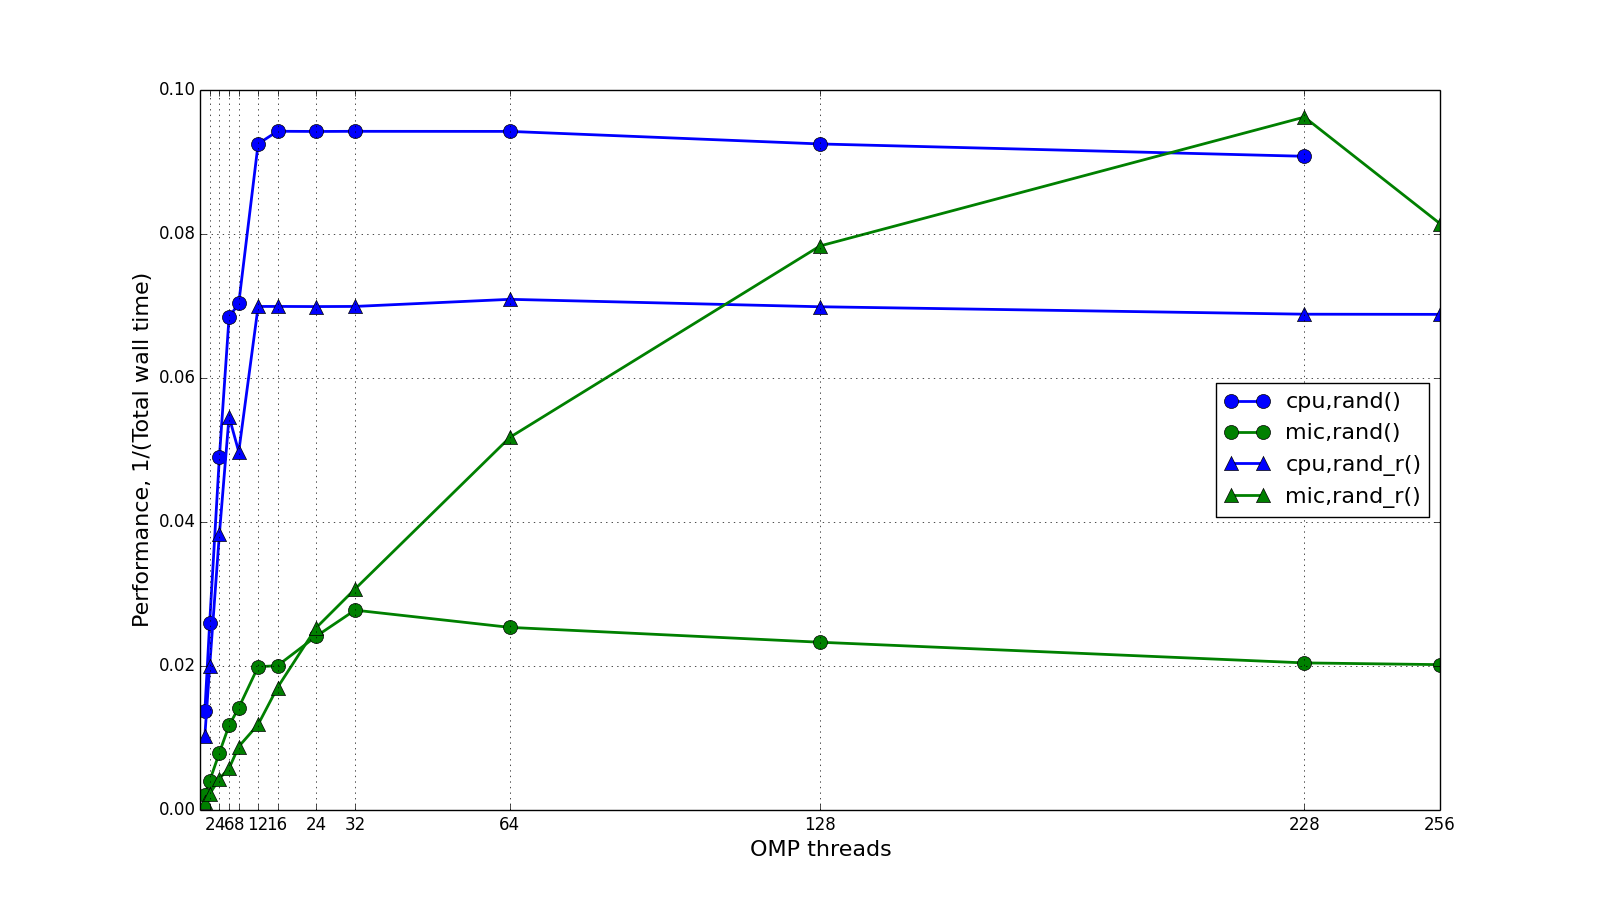
\includegraphics[width=0.8\textwidth] {img/mic/perf_rand_r.png}
  \caption{Performance using different random number generators.}
\end{figure}

  We also tested other more advanced RNGs in our code, such as Mersenne Twister, 
and PCG. They offer better statistical quality in the pseudo random number sequence,
and also have great multi-threading efficiency. However, the overall performance
gain is not significant, since the thread-safe RNG itself is not very time consuming
comparing to other parts of the code. 

\item Move memory allocation out of the OpenMP region
 In our implementation, the hybridization matrix needs to be updated for each 
accepted Monte Carlo move, and the size of the matrix depends on the number of 
segments in each channel. In addition to the old and updated matrices, temporary
storage for the intermediate matrices used in the fast update process are also
required. 

We find that the repeated allocation and free of memory used for the
said matrices poses a huge performance penalty. A better practice would be 
allocating all the space for the matrices before the OpenMP region, and free 
after the threads join. This sets a limit on the max size of the matrices. For
a low temperature, more segments are expected, which means the size of the matrices
would be bigger, and thus a larger space needs to be assigned. 

\begin{figure}
  \centering
  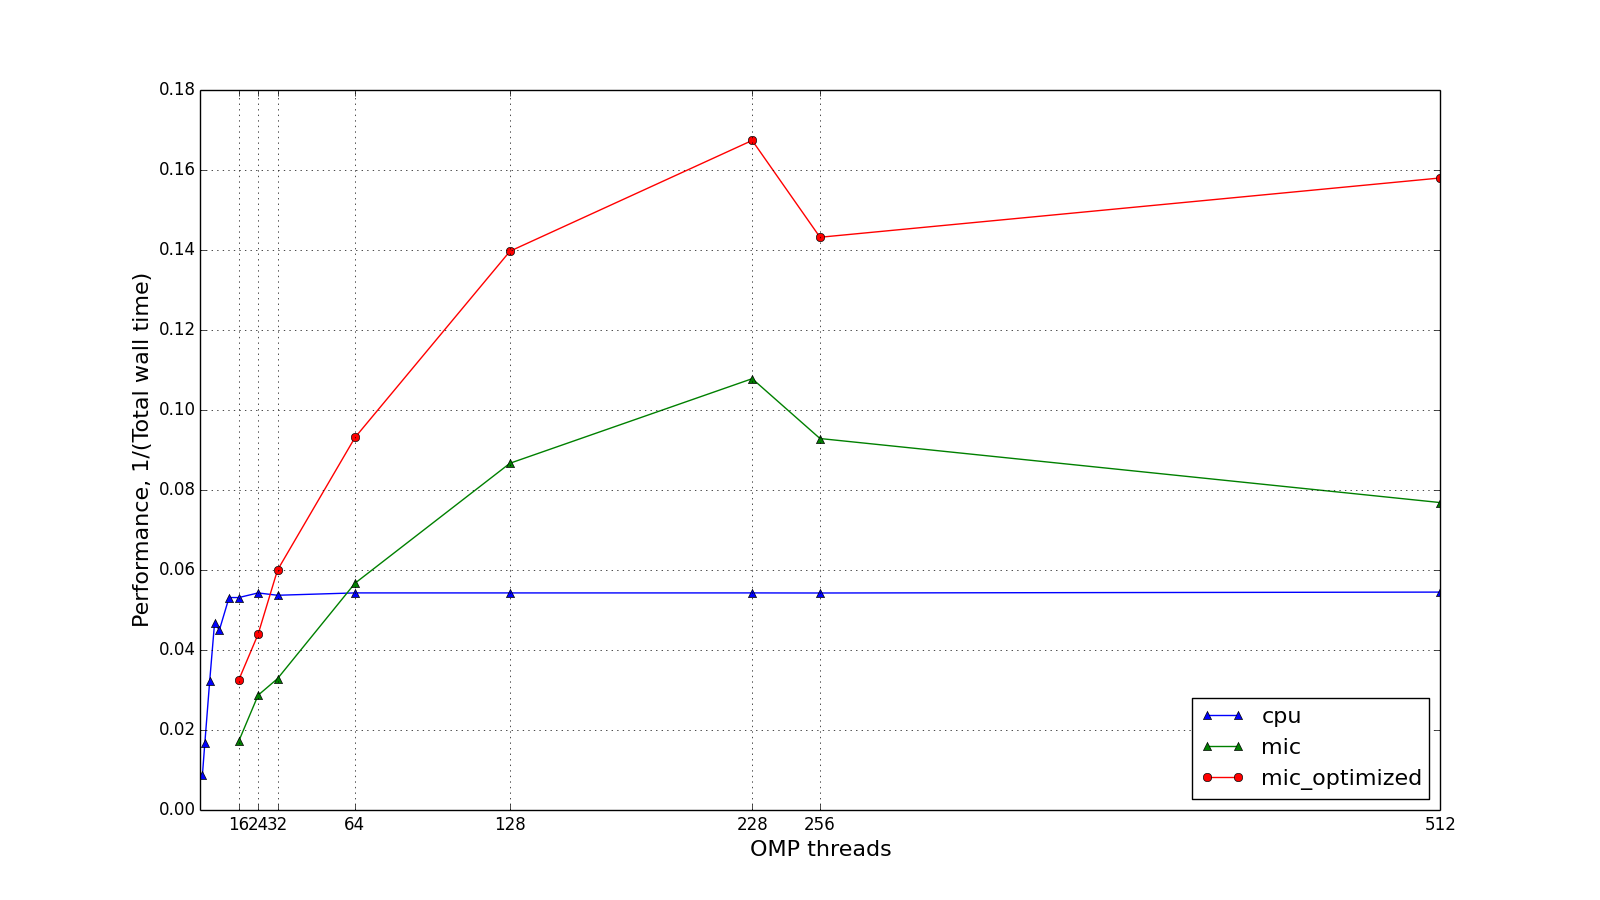
\includegraphics[width=0.8\textwidth] {img/mic/memory.png}
  \caption{Performance before and after memory allocation optimization for MIC.}
\end{figure}


\item Improve data access pattern in kernel by
\begin{itemize}
  \item Separating loops to avoid cache bank conflict
  \item Interchanging loops to guarantee Unit-Stride Access
  \item Aligning elements in array
  \item Enhancing matrix storage
\end{itemize}
\end{itemize}
With these optimization methods, we improved CPI rate, L1 hit ratio, and 
vectorization intensity. We achieved more than two times speed up comparing to 
original CPU code.


%\section{Dynamic Hubbard Models}
%\label{ssec:hyb-mod}

\section{Preliminary results}
We benchmark our CTQMC solver with another Hirsch Fye code and compare the results,
as shown in Fig.\ref{fig:u2}. This verifies that we can match the results of 
other impurity solvers.

\begin{figure}
  \centering
  \label{fig:u2}
  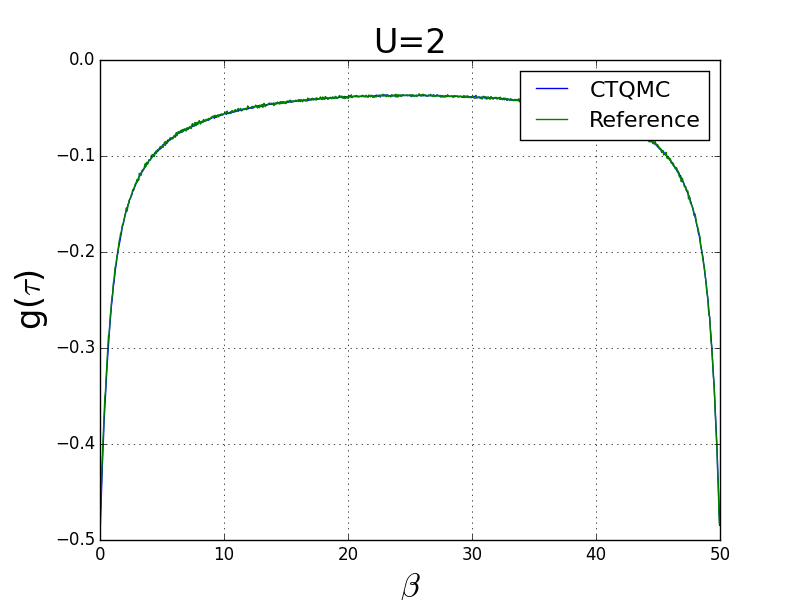
\includegraphics[width=0.8\textwidth] {img/U=2.png}
  \caption{Results for $G(\tau)$ on Anderson Model, from our code comparing with
weak coupling results.
Here $\beta = 50, U = 2, \mu = −1, v^2 = 0.156, D = 1, \Delta = v^2(log(i\omega + D) − log(i\omega − D))$}
\end{figure}



\section{Discussions\label{sec:hyb-concl}}

Although the formalism shown in \ref{sec:hyb-alg} is derived for single 
impurity Anderson model, the CT-HYB algorithm can be extended to more orbitals,
or other models easily, by changing the $H_\textrm{loc}$ term in the Hamiltonian 
and treating the term exactly. For example, we can easily extend the code to two
orbitals, and use exact diagonalization to calculate the contribution of the 
local term. For more orbitals, a Krylov solver \cite{PhysRevB.80.235117} can be used to reduce the cost of
trace computation.

One of the possible application of the solver is the Dynamical Hubbard Models. 
The Dynamical Hubbard models contains the idea of break the electron-hole 
symmetry, due to the insufficiency of conventional Hubbard model in describing 
some scenarios in real materials, where important physics happens in transport 
and other process. With the new methods applied, we hope to seek physics 
explanation to problems such as high Tc superconductivity. 

%%% Local Variables:
%%% mode: latex
%%% TeX-master: "../thesis"
%%% End:
